\documentclass[]{beamer}

\usepackage[utf8x]{inputenc}


% opciones para la presentacion
\usetheme{Warsaw}
% \usetheme{classic}

% multifiguras
\usepackage{subcaption}

% multilinea en tablas
\usepackage{multirow}

% texto "parado"
\usepackage{rotating}

% color de fondo en celdas
\usepackage{color, colortbl}
\newcommand{\pricomp}[2]{\only<1>{#2}\only<2>{\cellcolor{#1}#2}\only<3>{#2}}
\newcommand{\prisegcomp}[3]{\only<1>{#3}\only<2>{\cellcolor{#1}#3}\only<3>{\cellcolor{#2}{#3}}}
\newcommand{\segcomp}[2]{\only<1>{#2}\only<2>{#2}\only<3>{\cellcolor{#1}#2}}
\newcommand{\video}[1]{
    \begin{center}
        \href{run:#1}{
            
\includegraphics[width=1cm]{img/play.jpeg}
        }
    \end{center}
}
% Cuadro de texto de color
\usepackage{xcolor}

% Codigo
\usepackage{algorithm}
\usepackage{algpseudocode}

% Link a un archivo: \href{run:videos/desk_1.ogv}{\color{red}{DEMO}}


% datos de la presentacion
\title{Seguimiento de objetos en secuencias de imágenes RGB-D}
\subtitle{Tesis de licenciatura}
\institute{Facultad de Ciencias Exactas y Naturales}
\date[18/03/15]{Miércoles 18 de Marzo de 2015}
\author{Mariano Bianchi}


\begin{document}


\maketitle
% comentar como va a estar organizada la charla
%--- Next Frame ---%

%%%%%%%%%%%%%%%%%%%%%%%%%%
%%%%%%%%%%%%%%%%%%%%%%%%%%
\section{Introducción}
% \begin{frame}[t]{Si nos organizamos...}
%     \tableofcontents
%
% \end{frame}
% %--- Next Frame ---%

\subsection{Vamos por partes... del título}
\begin{frame}{}
    \textbf{\fcolorbox{red}{white}{Seguimiento} de objetos en secuencias de imágenes RGB-D}
    % El comportamiento esperado de un método de seguimiento es obtener para
    % cada imagen de una secuencia de imágenes o video la ubicación de un
    % objeto en algún eje de coordenadas elegido
    \begin{figure}[t]
        \centering
        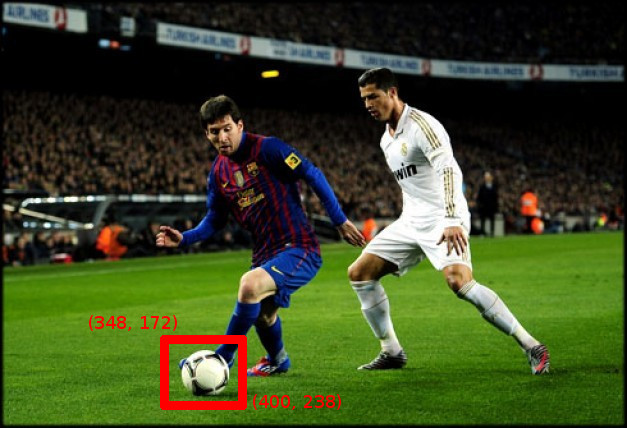
\includegraphics[scale=0.45]{img/seguimiento_ejemplo.jpg}
    \end{figure}
\end{frame}
%--- Next Frame ---%



\begin{frame}{}
    \textbf{Seguimiento de \fcolorbox{red}{white}{objetos} en secuencias de imágenes RGB-D}
    \begin{figure}[t]
        \centering
        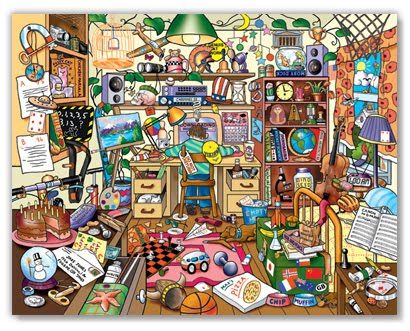
\includegraphics[scale=0.6]{img/escena_con_objetos.jpg}
    \end{figure}
\end{frame}
%--- Next Frame ---%



\begin{frame}{}
    \textbf{Seguimiento de objetos en \fcolorbox{red}{white}{secuencias de imágenes} RGB-D}
    % Puede ser un video, una ráfaga de imágenes tomada con una cámara de fotos
    \begin{columns}
        \begin{column}{3cm}
            \begin{figure}[t]
                \centering
                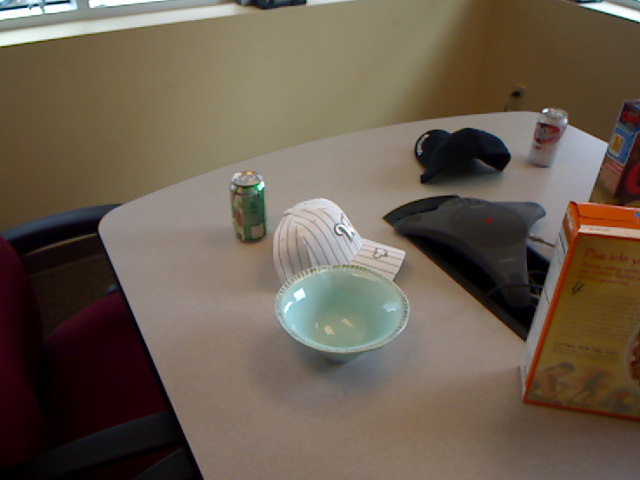
\includegraphics[width=\textwidth]{img/rafaga/1.png}
            \end{figure}
        \end{column}

        \begin{column}{0.5cm}
            \centering
            $\rightarrow$
        \end{column}

        \begin{column}{3cm}
            \begin{figure}[t]
                \centering
                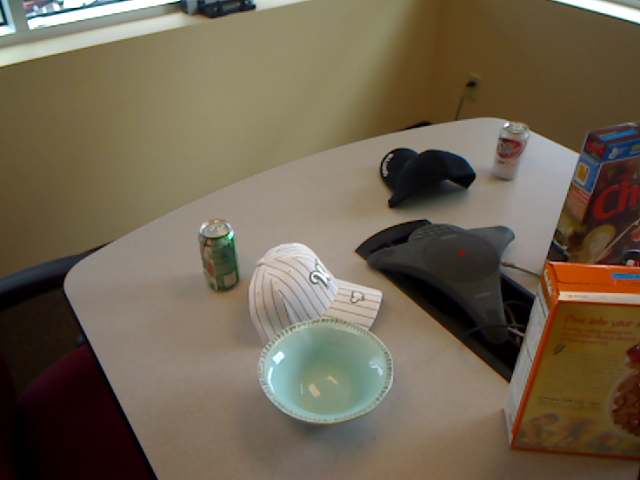
\includegraphics[width=\textwidth]{img/rafaga/2.png}
            \end{figure}
        \end{column}

        \begin{column}{0.5cm}
            \centering
            $\rightarrow$
        \end{column}

        \begin{column}{3cm}
            \begin{figure}[t]
                \centering
                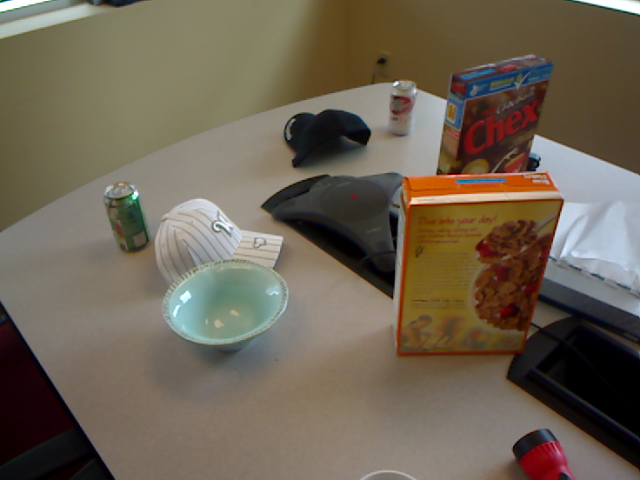
\includegraphics[width=\textwidth]{img/rafaga/3.png}
            \end{figure}
        \end{column}

    \end{columns}

    \begin{columns}
        \begin{column}{3cm}
            \begin{figure}[t]
                \centering
                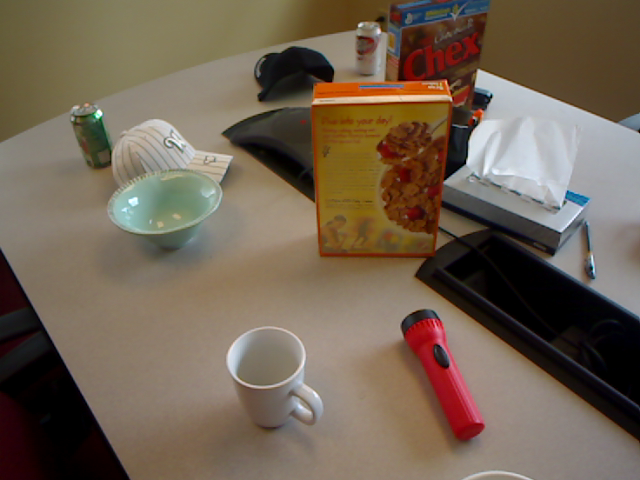
\includegraphics[width=\textwidth]{img/rafaga/4.png}
            \end{figure}
        \end{column}

        \begin{column}{0.5cm}
            \centering
            $\rightarrow$
        \end{column}

        \begin{column}{3cm}
            \begin{figure}[t]
                \centering
                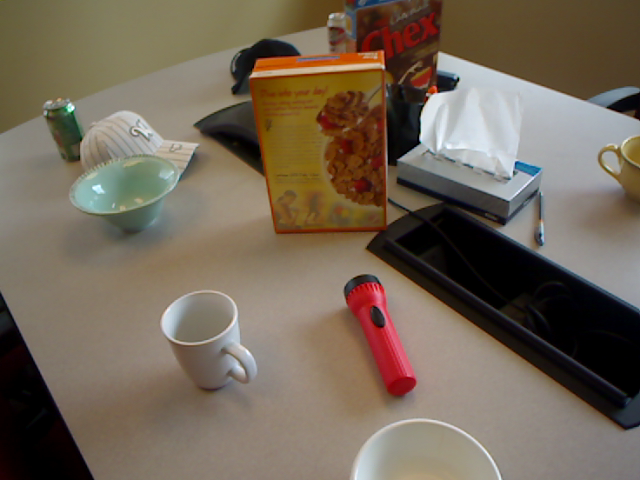
\includegraphics[width=\textwidth]{img/rafaga/5.png}
            \end{figure}
        \end{column}

        \begin{column}{0.5cm}
            \centering
            $\rightarrow$
        \end{column}

        \begin{column}{3cm}
            \begin{figure}[t]
                \centering
                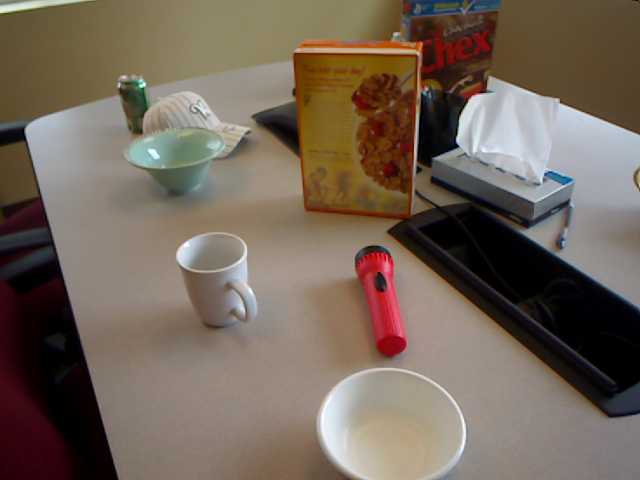
\includegraphics[width=\textwidth]{img/rafaga/6.png}
            \end{figure}
        \end{column}

    \end{columns}
    \video{videos/meeting_small.avi}
\end{frame}
%--- Next Frame ---%



\begin{frame}
    \textbf{Seguimiento de objetos en secuencias de \fcolorbox{red}{white}{imágenes RGB}-D}
    % Una imagen RGB-D está compuesta por dos partes. Una de ellas es una
    % imagen RGB
    % Las imágenes RGB son las más comunes y que todos conocen. Es simplemente
    % una fotografía. RGB significa Red Green Blue, que son los colores
    % primarios lumínicos (en el dominio de la luz), es decir, que el resto de los colores puede definirse
    % con una combinación de estos tres colores
    \begin{columns}
        \begin{column}{8cm}
            \begin{figure}[t]
                \centering
                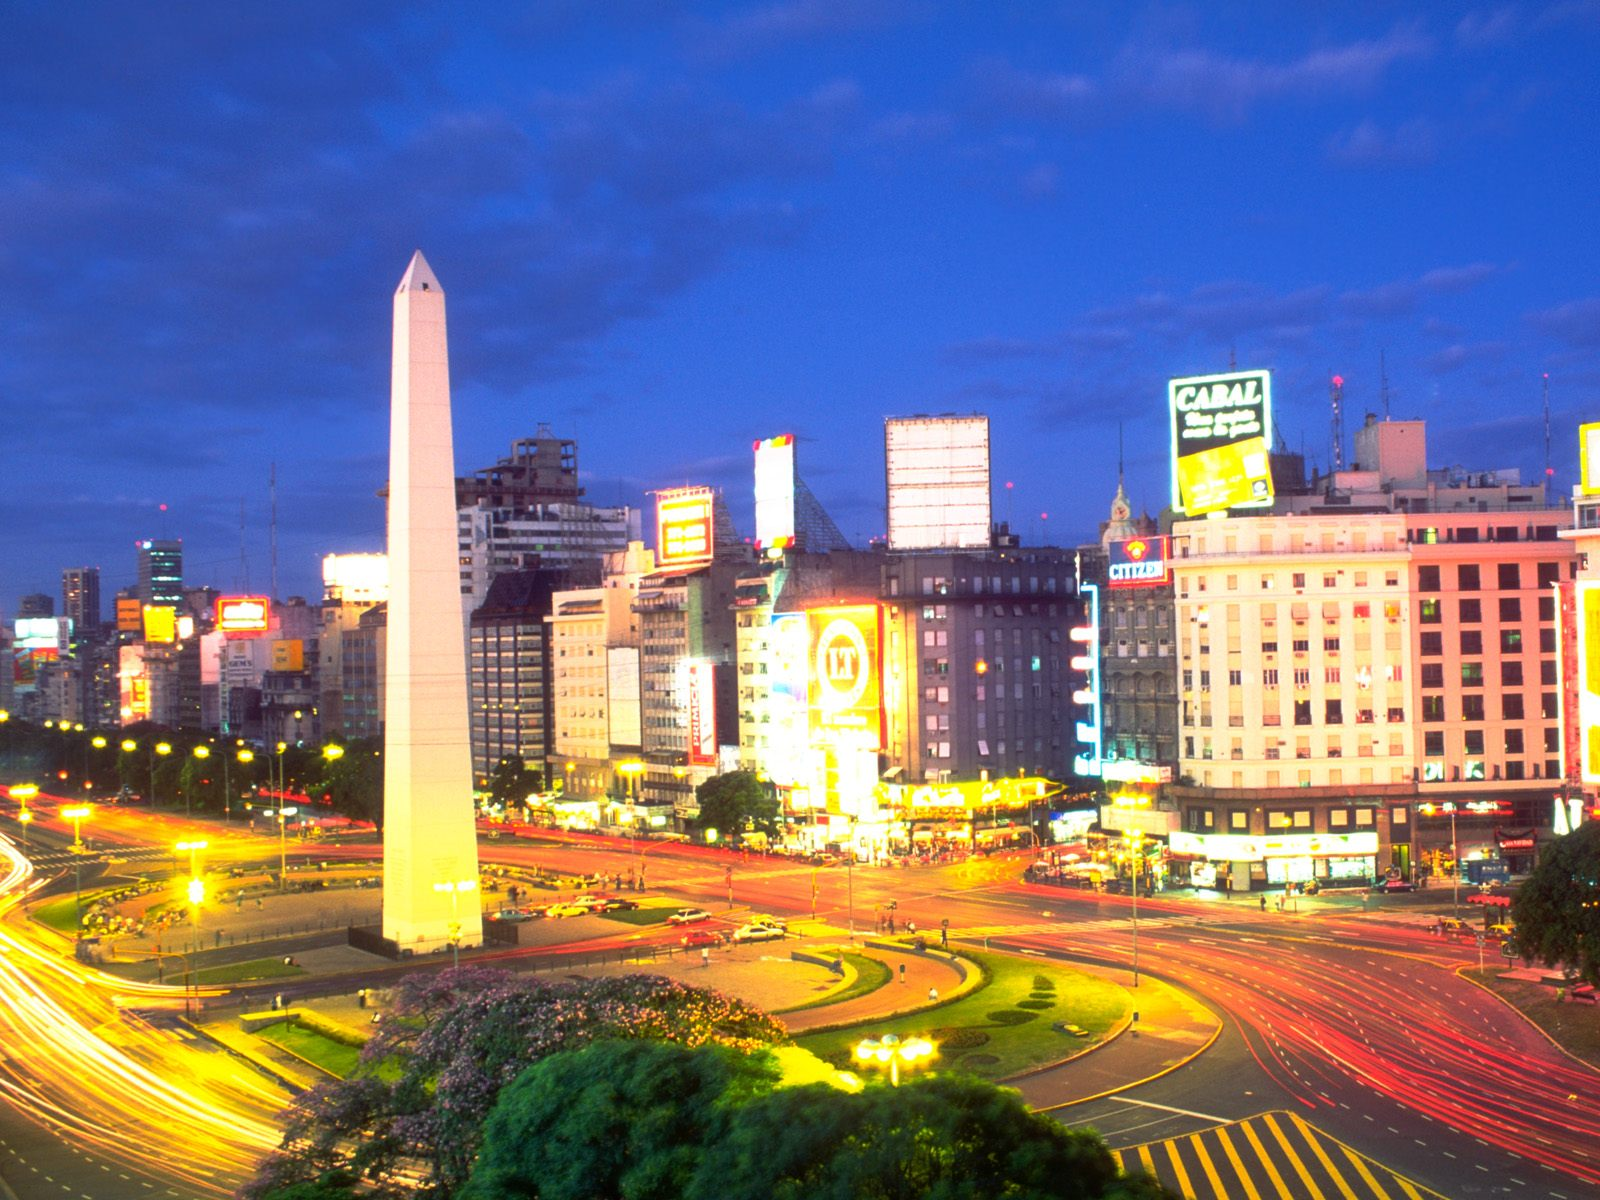
\includegraphics[width=\textwidth]{img/rgb.jpg}
            \end{figure}
        \end{column}
        \begin{column}{3cm}
            \begin{figure}[t]
                \centering
                
\includegraphics[width=\textwidth]{img/pixel.png}
            \end{figure}
        \end{column}
    \end{columns}

\end{frame}
%--- Next Frame ---%

\begin{frame}{}
    \textbf{Seguimiento de objetos en secuencias de \fcolorbox{red}{white}{imágenes} RGB-\fcolorbox{red}{white}{D}}
    % Un sensor RGB-D cuenta con una cámara tipo webcam que otorga imagenes RGB,
    % un proyector infrarrojo y una cámara infrarroja. El proyector dibuja un patrón
    % conocido en la escena, que al ser infrarrojo es invisible al ojo humano.
    % Luego la cámara infrarroja captura ese patrón proyectado y utilizando algoritmos
    % de luz estructurada junto con las distancias conocidas entre la cámara y proyector
    % infrarrojo se puede obtener la profundidad para cada pixel de la escena.
    % MOSTRAR SENSOR RGB-D, contar como funciona y mostrar con el pcl\_viewer una nube de puntos y una imagen RGB-D
    \begin{figure}[t]
        \centering
        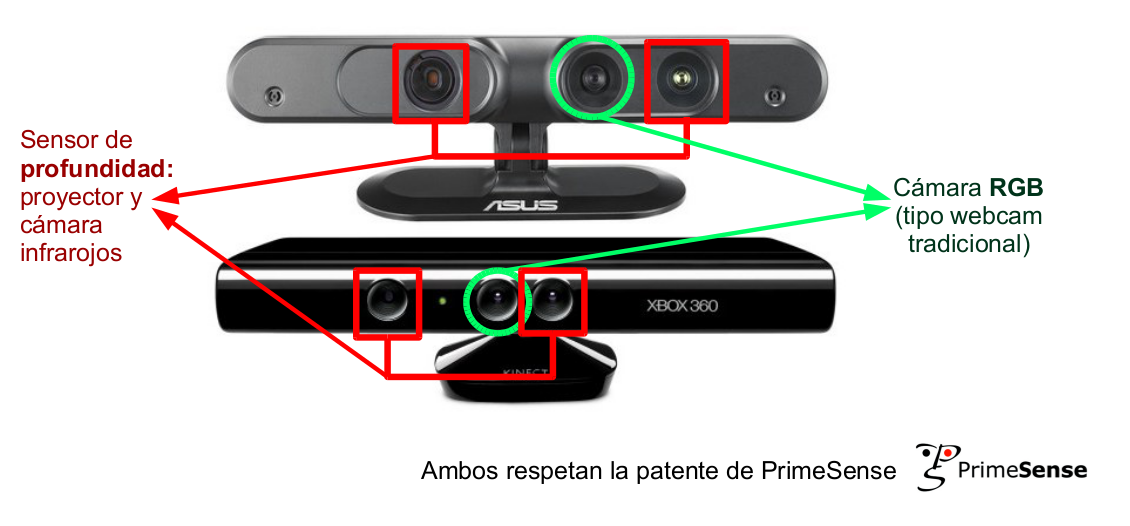
\includegraphics[width=\textwidth]{img/sensores_rgbd.png}
    \end{figure}
    \begin{columns}
        \begin{column}{2cm}
            \video{videos/desk_1.ogv}
        \end{column}
        \begin{column}{2cm}
            \video{videos/rgbd.ogv}
        \end{column}
    \end{columns}




\end{frame}
%--- Next Frame ---%


\subsection{Aplicaciones}
\begin{frame}{Aplicaciones} % si pongo la opcion [t] el texto empieza desde arriba

    % El seguimiento de objetos en secuencias de imágenes tiene muchas aplicaciones.
    % Desde hace muchos años es un tema de estudio dentro del área de procesamiento de imágenes
    % y aún se siguen desarrollando más y mejores herramientas para este fin.
    % Varias de sus aplicaciones nos las cruzamos todos los días sin darnos cuenta,
    % como por ejemplo, la generación de estadísticas deportivas. BLABLABLA

    % Permite generar estadísitcas deportivas midiendo la distancia recorrida por
    % jugadores de futbol, tiros al arco, goles, faltas realizadas, etc
    \begin{figure}[t]
        \centering
        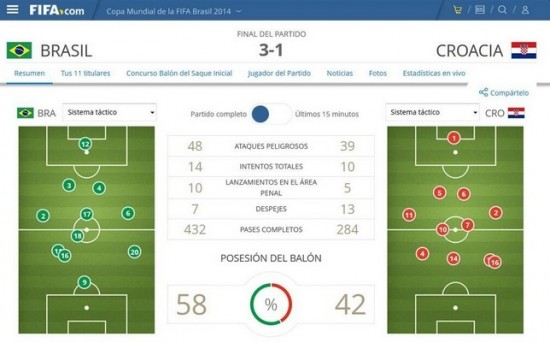
\includegraphics[scale=0.5]{img/estadistica.jpg}
    \end{figure}
\end{frame}

\begin{frame}{Aplicaciones}
    % Permite que un robot sepa de que manera tomar un objeto y usarlo como
    % herramienta de trabajo
    \begin{figure}[t]
        \centering
        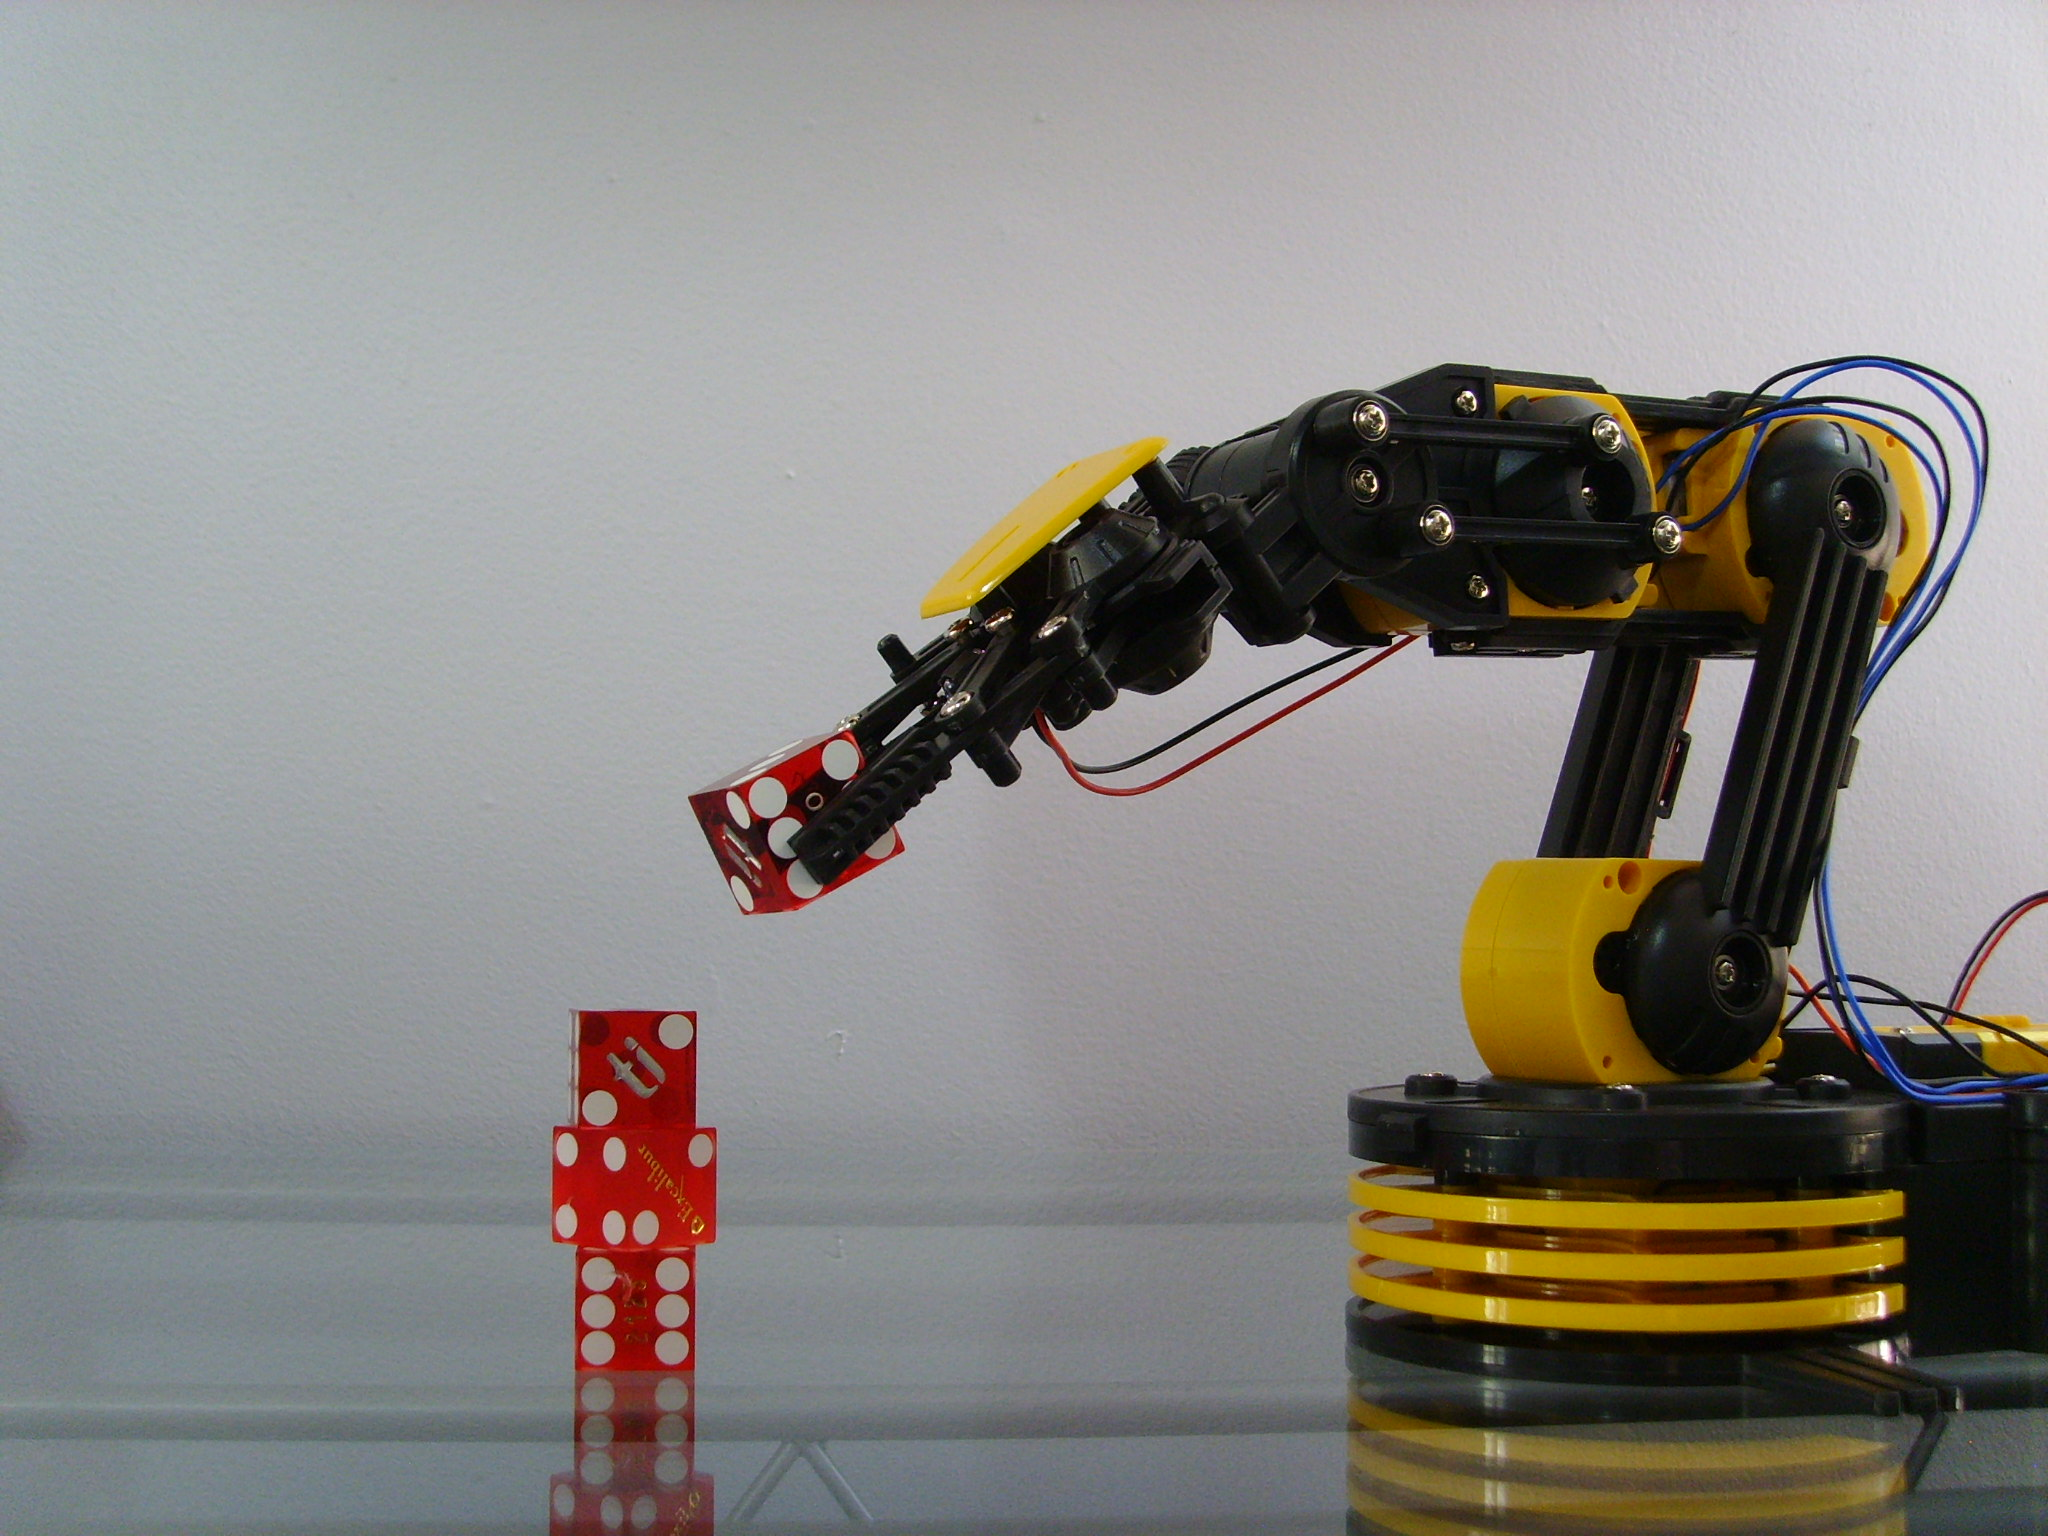
\includegraphics[scale=0.12]{img/robot.jpg}
    \end{figure}
\end{frame}


\subsection{Objetivos}
\begin{frame}{Objetivos}
    % Decir en la slide anterior: ahora que todos sabemos de que trata este trabajo, ¿por qué estudiamos este tema?
    % Lo estudiamos por varios motivos. Principalmente nuestra idea fue tener un sistema de seguimiento completo en RGB-D en donde sea sencillo probar distintos métodos de seguimiento. En segunda instancia queríamos comparar el funcionamiento de métodos de seguimiento clásicos en RGB y en profundidad y poder contrastar resultados, entender las ventajas y desventajas de cada uno y saber en qué casos es preferible RGB por sobre profundidad y vice versa.
    % Además, nos encontramos con falta de información en la literatura sobre el comportamiento de un sistema de seguimiento RGB-D completo.

    % Vamos entonces a meternos un poco más en el foco de estudio de este trabajo. Hasta ahora veníamos hablando de seguimiento unicamente y en esta ultima parte hablé de un sistema de seguimiento completo. ¿Qué es un sistema de seguimiento?
    \begin{enumerate}
        \item Implementamos, estudiamos y evaluamos un sistema de seguimiento RGB-D, enfocándonos en la etapa de seguimiento
        \item Comparamos métodos de seguimiento en RGB y en profundidad y analizamos sus ventajas y desventajas
        \item Análisis en detalle de un sistema de seguimiento RGB-D completo, poco común en la literatura
    \end{enumerate}
\end{frame}
%--- Next Frame ---%


%%%%%%%%%%%%%%%%%%%%%%%%%%
%%%%%%%%%%%%%%%%%%%%%%%%%%
\section{Sistemas de seguimiento}
\begin{frame}[t]{Sistema de seguimiento}

    % IDEA DE ESTE SLIDE: motivaciones, por que la separacion de los metodos,
    % comparar metodos rgb y d

    % Partiendo del esquema antes visto como base de nuestro sistema de seguimiento
    % nos propusimos desarrollar un sistema de seguimiento RGB, uno en profundidad
    % y luego utilizar lo mejor de cada uno para crear un sistema RGB-D que
    % combine lo mejor de cada uno
    % El motivo por el cual desarrollamos 2 sistemas por separado es para poder
    % cuantificar las diferencias entre usar alguno de esos sistemas por separado
    % o uno que los combine y decidir cual se comporta mejor en general o en cada
    % situacion en particular
    % \begin{itemize}
    %     \item Sistema RGB completo y funcional
    %     \item Sistema en profundidad completo y funcional
    %     \item Combinarlos de la mejor manera posible
    %     \item Obtener resultados comparables frente a métodos existentes
    % \end{itemize}


    % Un sistema de seguimiento tiene esta pinta. Posee 3 etapas bien definidas

    \begin{figure}[t]
        \centering
        \vspace{-13pt}
        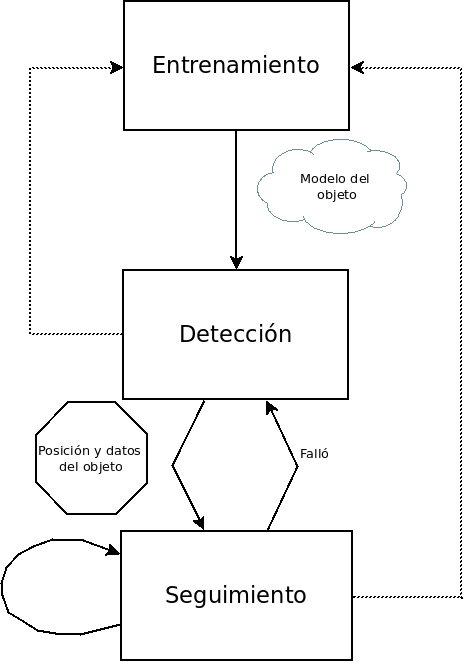
\includegraphics[scale=0.3]{img/esquema_seguimiento.png}
    \end{figure}
\end{frame}
%--- Next Frame ---%


\subsection{Sistema RGB}
\begin{frame}[fragile]{Sistema RGB}
    \begin{columns}
        \begin{column}{0.4\textwidth}
            \begin{figure}
                \centering
                \vspace{-25pt}
                % \hspace*{-20pt}
                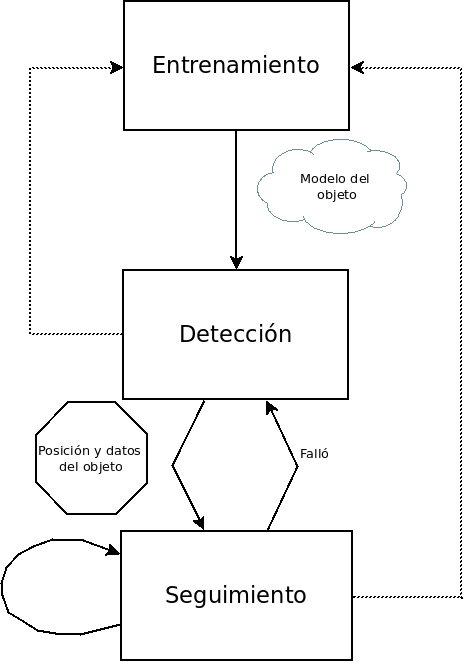
\includegraphics[scale=0.3]{img/esquema_seguimiento.png}
            \end{figure}
        \end{column}

        \begin{column}{0.6\textwidth}
            % ENTRENAMIENTO
            \only<1>{
                \begin{center}
                    \textbf{Entrenamiento}: \\ \textit{Recolección de templates}
                \end{center}

                \begin{figure}
                	\centering
                	\begin{subfigure}[b]{0.4\textwidth}
                		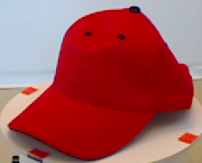
\includegraphics[width=\textwidth]{img/templates/0_crop.png}
                	\end{subfigure}
                	\quad
                	\begin{subfigure}[b]{0.4\textwidth}
                		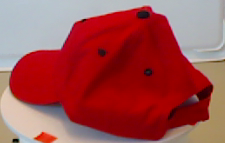
\includegraphics[width=\textwidth]{img/templates/90_crop.png}
                	\end{subfigure}

                	\begin{subfigure}[b]{0.4\textwidth}
                		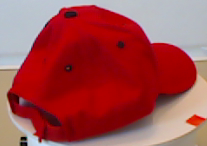
\includegraphics[width=\textwidth]{img/templates/180_crop.png}
                	\end{subfigure}
                	\quad
                	\begin{subfigure}[b]{0.4\textwidth}
                		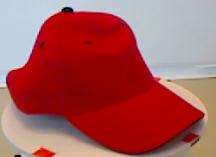
\includegraphics[width=\textwidth]{img/templates/270_crop.png}
                	\end{subfigure}
                \end{figure}
            }
            % DETECCION
            % \begin{block}{Pasos del algoritmo de template matching}
            %     Para cada template proveniente del entrenamiento y para cada pixel de la escena, seguir estos pasos:
            %     \begin{enumerate}
            %         \item Tomar un rectángulo de la escena del tamaño del template cuya esquina superior izquierda sea el pixel actual
            %         \item Compararlo con el template (ejemplo: diferencia cuadrática pixel por pixel)
            %         \item Si la comparación está por debajo de un umbral predefinido y es el mejor valor encontrado, guardar la ubicación del pixel
            %     \end{enumerate}
            %     Una vez recorrida toda la imagen, se devuelve la ubicación del ``mejor recuadro''. Si no se encontró ninguno por debajo del umbral, se indica que no se encontró el objeto en la imagen.
            % \end{block}
            \only<2>{
                \vspace{-15pt}
                \begin{center}
                    \textbf{Detección}: \\ \textit{Template matching}
                \end{center}

                \begin{figure}[t]
                    \centering
                    \vspace{-15pt}
                    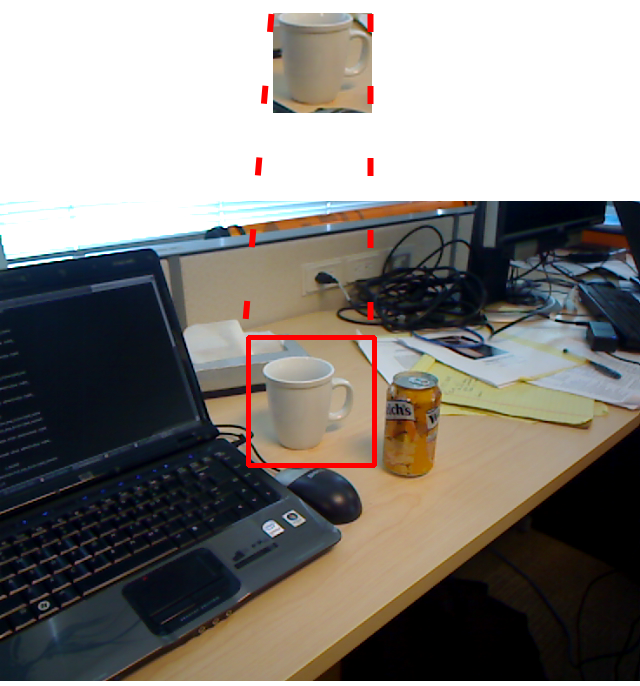
\includegraphics[width=0.8\textwidth]{img/template_matching/template_matching_marcado.png}
                \end{figure}
            }
            \only<3>{
                \vspace{-15pt}
                \begin{center}
                    \textbf{Detección}: \\ \textit{Template matching}
                \end{center}

                \footnotesize
                \begin{algorithmic}
                    \Function{$custom\_t\_match$}{$templates, scene$}
                        \For{tmp in templates}
                            \For{scale in scales}
                                \State $rescale(tmp, scale)$
                                \State $template\_matching(tmp, scene)$
                            \EndFor
                        \EndFor
                        \State \Return $best\_template\_matching$
                    \EndFunction
                \end{algorithmic}
                \normalsize
            }
            % SEGUIMIENTO
            \only<4>{
                \begin{center}
                    \textbf{Seguimiento}: \\ \textit{Comparación de histogramas}
                \end{center}
                \begin{figure}[t]
                	\centering
                    \vspace{-15pt}
                	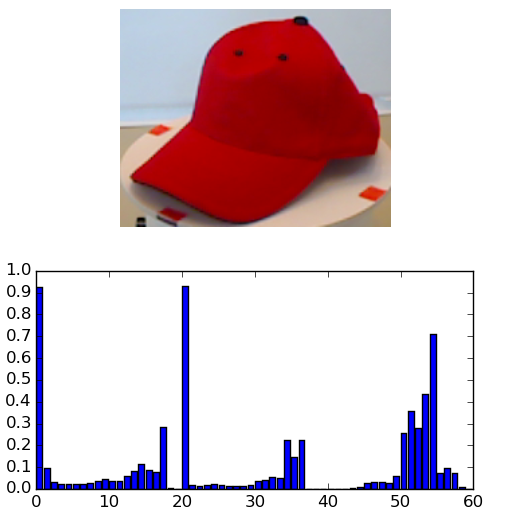
\includegraphics[width=0.8\textwidth]{img/template_histogram.png}
                \end{figure}
            }
        \end{column}

    \end{columns}

\end{frame}
%--- Next Frame ---%

\begin{frame}[t]{Veamos un ejemplo!}
    \begin{figure}[t]
        \centering
        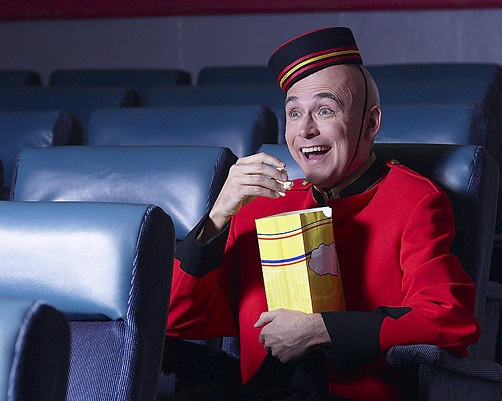
\includegraphics[scale=0.5]{img/pochoclos/comiendo_1.jpg}
    \end{figure}
    \video{videos/seguimiento_rgb.avi}
\end{frame}
%--- Next Frame ---%



\subsection{Sistema en profundidad}
\begin{frame}{¿Cómo se ve un video en profundidad?}
    \begin{columns}
        \begin{column}{0.8\textwidth}
            \begin{figure}[t]
                \vspace{-15pt}
                \centering
                
\includegraphics[scale=0.4]{img/anteojos/poner_anteojos_3d_5.jpg}
            \end{figure}
        \end{column}
        \begin{column}{0.15\textwidth}
            \video{videos/video_depth.ogv}
        \end{column}
    \end{columns}
\end{frame}
%--- Next Frame ---%


\begin{frame}[fragile]{Sistema en profundidad}
    \begin{columns}
        \begin{column}{5cm}
            \begin{figure}
                \centering
                \vspace{-15pt}
                % \hspace*{-20pt}
                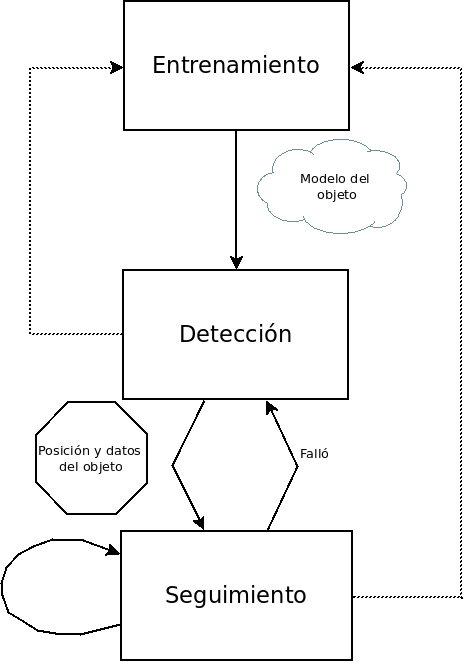
\includegraphics[scale=0.3]{img/esquema_seguimiento.png}
            \end{figure}
        \end{column}

        % Esta columna vacia esta para separar las otras 2 columnas
        \begin{column}{0.5cm}
        \end{column}

        \begin{column}{5cm}
            % ENTRENAMIENTO
            \only<1>{
                \begin{center}
                    \textbf{Entrenamiento}: \\ \textit{Nube de puntos}
                \end{center}
                \vspace{-20pt}
                \begin{figure}
                	\begin{subfigure}[b]{\textwidth}
                        \centering
                		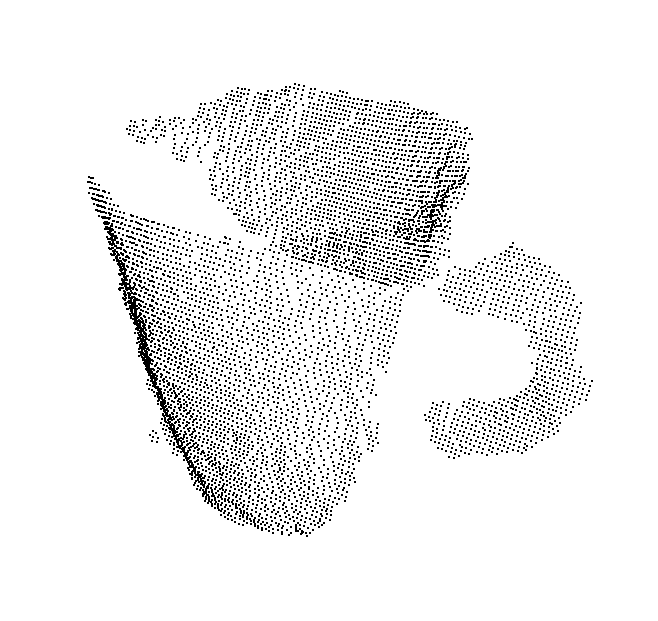
\includegraphics[scale=0.1]{img/nubes/taza_02.png}
                	\end{subfigure}
                	\quad
                	\begin{subfigure}[b]{\textwidth}
                        \centering
                		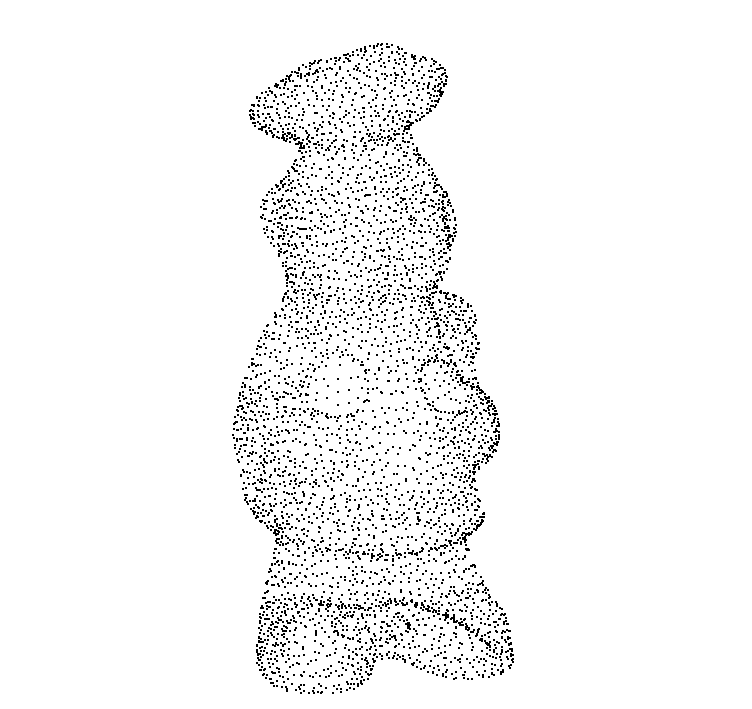
\includegraphics[scale=0.1]{img/nubes/chef_01.png}
                	\end{subfigure}
                \end{figure}
            }
            % DETECCION:
            % Explicar que se establecen correspondencias usando "Alignment prerejective".
            % Estimo correspondencias, busco la transformacion con RANSAC y refino con ICP

            % Tanto RANSAC como ICP son métodos de estimación de pose y alineación
            % Toman una nube de puntos "query" y otra "escena" y estiman una
            % transformacion que alinee de la mejor manera "query" segun las
            % coordenadas de "escena"
            % La diferencia principal entre ambos métodos es que RANSAC es robusto
            % frente a outliers. Por esta razón se utiliza primero RANSAC y luego
            % para refinar el resultado, ICP
            \only<2>{
                \begin{center}
                    \textbf{Detección}: \\ \textit{Alignment Prerejective e ICP}
                \end{center}

                \vspace{-10pt}
                \begin{figure}[t]
                    \centering
                    \begin{subfigure}[b]{0.7\textwidth}
                        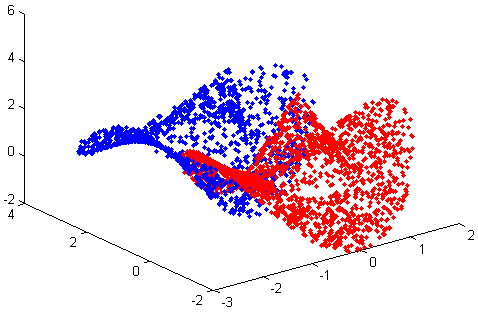
\includegraphics[width=\textwidth]{img/alineacion/icp_ini.png}
                    \end{subfigure}
                    \quad
                    \begin{subfigure}[b]{0.7\textwidth}
                        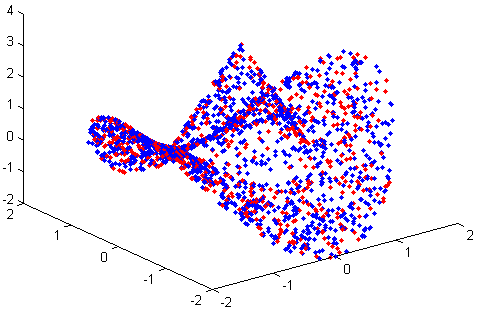
\includegraphics[width=\textwidth]{img/alineacion/icp_fin.png}
                    \end{subfigure}
                \end{figure}
            }
            % SEGUIMIENTO
            %
            \only<3>{
                \begin{center}
                    \textbf{Seguimiento}: \\ \textit{ICP}
                \end{center}
                % \tiny
                \footnotesize
                \begin{algorithmic}
                    \Function{icp}{$obj, scene$}
                    	\Loop
                    		\State $get\_closest\_points()$
                    		\State $get\_transformation()$
                    		\State $transform(obj)$
                    		\State $sq\_dist \gets mean\_sq\_dist()$
                    	\EndLoop
                        \State \Return $obj, sq\_dist$
                    \EndFunction
                \end{algorithmic}
                \normalsize

                \begin{columns}
                    \begin{column}{2cm}
                        \video{videos/taza_pre_icp.ogv}
                    \end{column}
                    \begin{column}{2cm}
                        \video{videos/taza_post_icp.ogv}
                    \end{column}
                \end{columns}
            }
        \end{column}

    \end{columns}

\end{frame}
%--- Next Frame ---%


\begin{frame}[t]{Veamos un ejemplo!}
    \begin{figure}[t]
        \centering
        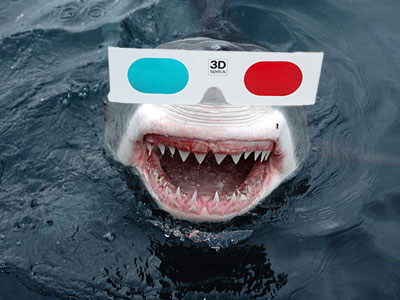
\includegraphics[scale=0.5]{img/anteojos/poner_anteojos_3d_7.jpg}
    \end{figure}
    \video{videos/seguimiento_depth.ogv}
\end{frame}
%--- Next Frame ---%


\subsection{Sistema RGB-D}
\begin{frame}{Sistema RGB-D}
    \begin{columns}
        \begin{column}{5cm}
            \begin{figure}
                \centering
                \vspace{-15pt}
                % \hspace*{-20pt}
                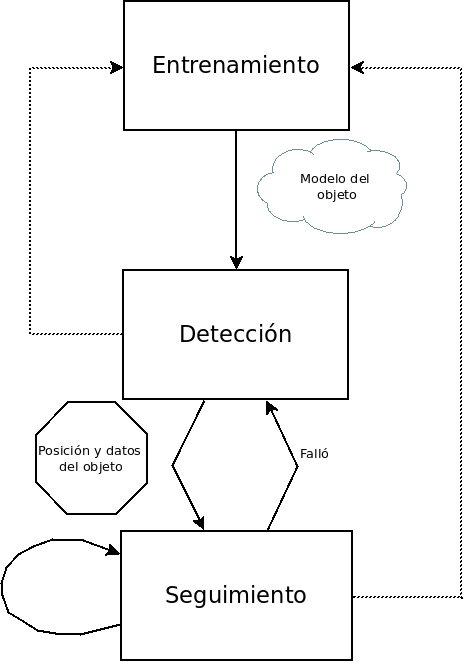
\includegraphics[scale=0.3]{img/esquema_seguimiento.png}
            \end{figure}
        \end{column}

        \begin{column}{0.5cm}
        \end{column}

        \begin{column}{5cm}
            % ENTRENAMIENTO
            \only<1>{
                \begin{center}
                    \textbf{Entrenamiento}: \\ \textit{Nube de puntos y templates}
                \end{center}
                \vspace{-20pt}
                \begin{figure}
                	\begin{subfigure}[b]{\textwidth}
                        \centering
                		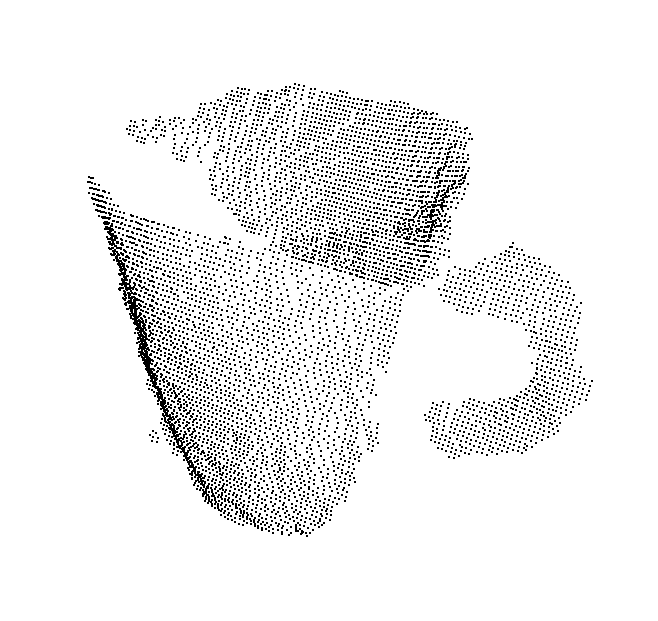
\includegraphics[scale=0.15]{img/nubes/taza_02.png}
                	\end{subfigure}
                	\quad
                	\begin{subfigure}[b]{\textwidth}
                        \centering
                		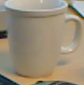
\includegraphics[scale=0.7]{img/templates/coffee_mug_5.png}
                	\end{subfigure}
                \end{figure}
            }
            % DETECCION
            % Tanto RANSAC como ICP son métodos de estimación de pose y alineación
            % Toman una nube de puntos "query" y otra "escena" y estiman una
            % transformacion que alinee de la mejor manera "query" segun las
            % coordenadas de "escena"

            % explicar que se establecen correspondencias usando "Alignment prerejective". Estimo correspondencias, busco la transformacion con RANSAC y refino con ICP

            % La diferencia principal entre ambos métodos es que RANSAC es robusto
            % frente a outliers. Por esta razón se utiliza primero RANSAC y luego
            % para refinar el resultado, ICP
            \only<2>{
                \begin{center}
                    \textbf{Detección}:
                \end{center}
                \begin{enumerate}
                    \item Template Matching
                    \item Alignment Prerejective
                    \item ICP
                \end{enumerate}
            }
            % SEGUIMIENTO
            %
            \only<3>{
                \begin{center}
                    \textbf{Seguimiento}:
                \end{center}
                \begin{enumerate}
                    \item ICP
                    \item Refinar usando comparación de histogramas
                \end{enumerate}
            }
        \end{column}

    \end{columns}

\end{frame}

\subsection*{}
\begin{frame}{¿Y ahora cómo seguimos?}
    % Pero para poder comparar los métodos entre si y saber cual funciona mejor
    % en que casos necesitamos tener una base de datos con información de
    % ground truth (la traducción sería de verdad absoluta) con la que podamos
    % corroborar el comportamiento de cada método y cada sistema

    % TODO: antes de esta slide comentar algo sobre lo que hicimos despues: una vez que tenemos los sistemas necesitabamos una base que tuviera información de rgb y profundidad, con objetos, escenas e info de ground truth

    % PONER UNA IMAGEN CON LOS SISTEMAS A LA IZQUIERDA, A LA DERECHA RESULTADOS Y EN EL MEDIO SIGNOS DE PREGUNTA
    % \begin{itemize}
    %     \item Analizamos los sistemas propuestos
    %     \item Comparamos los resultados arrojados por cada uno
    %     \item Definimos ventajas y desventajas
    % \end{itemize}
    \begin{figure}[t]
        \centering
        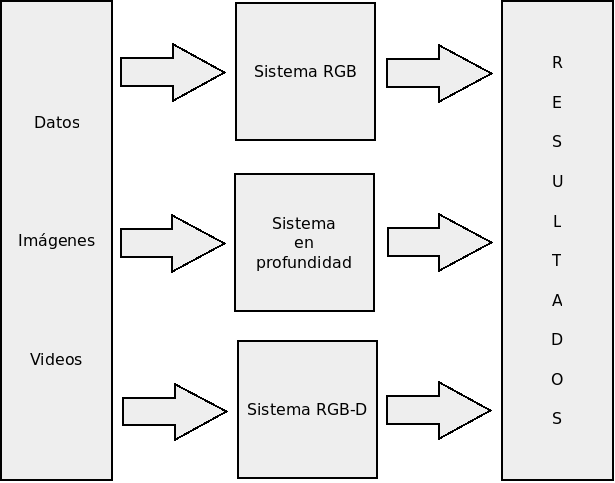
\includegraphics[scale=0.4]{img/diagrama_datos_sistema/datos_sistemas.png}
    \end{figure}

\end{frame}
%--- Next Frame ---%


%%%%%%%%%%%%%%%%%%%%%%%%%%
%%%%%%%%%%%%%%%%%%%%%%%%%%
\section{Resultados}
\subsection{Base de datos}
\begin{frame}{Base de datos}

    % Para poder cuantificar que tan bien funcionaron los métodos y compararlos
    % entre si utilizamos una BD de objetos y escenas de donde obtuvimos
    % información de ground truth (verdad absoluta)
    % La base tiene por un lado objetos, ordenados en diferentes categorías
    % y con distintas instancias por categoría. Por ejemplo: 5 tazas distintas
    % para la categoría tazas, 4 gorras en la categoría gorras
    % Para cada objeto tiene grabadas 3 escenas desde distintas alturas en donde
    % se filma al objeto girando sobre una base giratoria, se toman imagenes
    % cada 3 grados, se las segmenta tanto en RGB como en profundidad (nube de
    % puntos). Suman una totalidad de 300 obj
    % Además cuenta con 8 escenas en las cuales aparecen algunos de los objetos
    % de la base. Las escenas están anotadas frame por frame indicando la
    % ubicación del objeto o de los objetos en ese frame

    % Decir algo sobre que solo se mueve la cámara

    \begin{columns}[t]
        \begin{column}{5cm}
            \begin{itemize}
                \item 300 objetos de uso diario
                \item 51 categorías
                \item Segmentados en RGB y en profundidad
            \end{itemize}

            \begin{figure}
                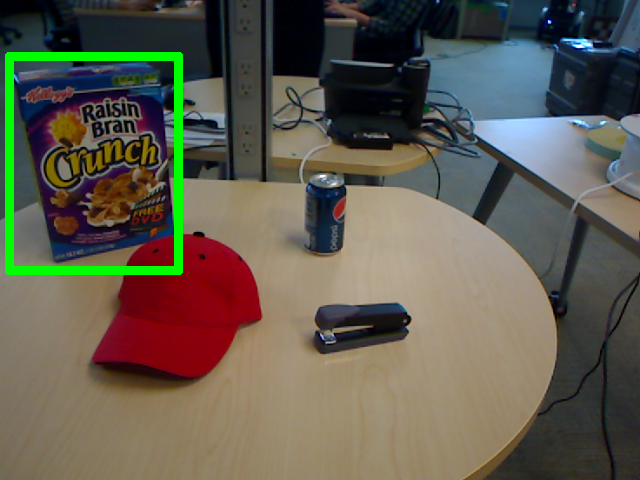
\includegraphics[width=0.8\textwidth]{img/base/scene_anotada.png}
            \end{figure}

        \end{column}
        \begin{column}{5cm}
            \begin{figure}
            	\centering
            	\begin{subfigure}{1.2cm}
            		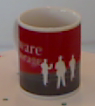
\includegraphics[width=\textwidth]{img/base/1.png}
            	\end{subfigure}
            	\begin{subfigure}{1.2cm}
            		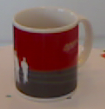
\includegraphics[width=\textwidth]{img/base/2.png}
            	\end{subfigure}
                \quad
                \quad
                \quad
                \quad
                \quad
                \quad
            	\begin{subfigure}{1.2cm}
            		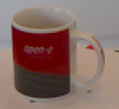
\includegraphics[width=\textwidth]{img/base/3.png}
            	\end{subfigure}
            	\begin{subfigure}{1.2cm}
            		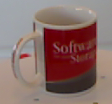
\includegraphics[width=\textwidth]{img/base/4.png}
            	\end{subfigure}
            \end{figure}

            \begin{itemize}
                \item 8 escenas
                \item Distintas instancias y categorías de objetos por escena
                \item \alert{\textbf{Anotadas}} en RGB
            \end{itemize}

        \end{column}
    \end{columns}
\end{frame}
%--- Next Frame ---%

\subsection{Selección de objetos y escenas para las pruebas}
\begin{frame}{Selección de objetos para las pruebas}
    \begin{figure}
        \centering
        \begin{subfigure}{0.3\textwidth}
            \centering
            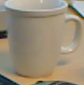
\includegraphics[scale=0.8]{img/templates/coffee_mug_5.png}
        \end{subfigure}
        \begin{subfigure}{0.3\textwidth}
            \centering
            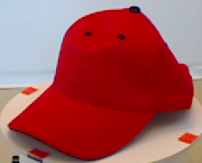
\includegraphics[scale=0.4]{img/templates/0_crop.png}
        \end{subfigure}
        \begin{subfigure}{0.3\textwidth}
            \centering
            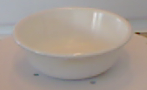
\includegraphics[scale=0.6]{img/templates/bowl.png}
        \end{subfigure}

        \begin{subfigure}{0.3\textwidth}
            \centering
            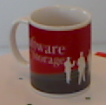
\includegraphics[scale=0.7]{img/templates/coffee_mug_1.png}
        \end{subfigure}
        \begin{subfigure}{0.3\textwidth}
            \centering
            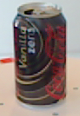
\includegraphics[scale=0.7]{img/templates/soda_can.png}
        \end{subfigure}
        \begin{subfigure}{0.3\textwidth}
            \centering
            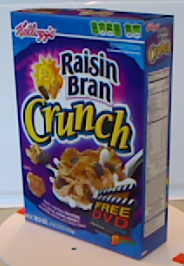
\includegraphics[scale=0.35]{img/templates/cereal_box.png}
        \end{subfigure}
    \end{figure}
\end{frame}
%--- Next Frame ---%

\begin{frame}{Selección de escenas para las pruebas}
    \begin{figure}
        \centering
        \begin{subfigure}{0.45\textwidth}
            \centering
            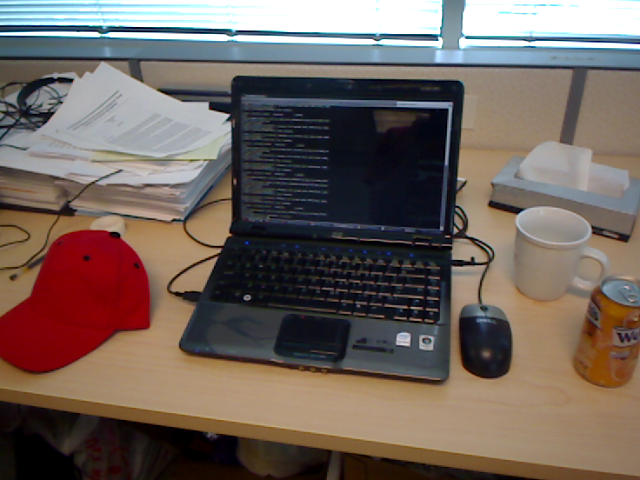
\includegraphics[scale=0.2]{img/escenas/desk_1.png}
        \end{subfigure}
        \begin{subfigure}{0.45\textwidth}
            \centering
            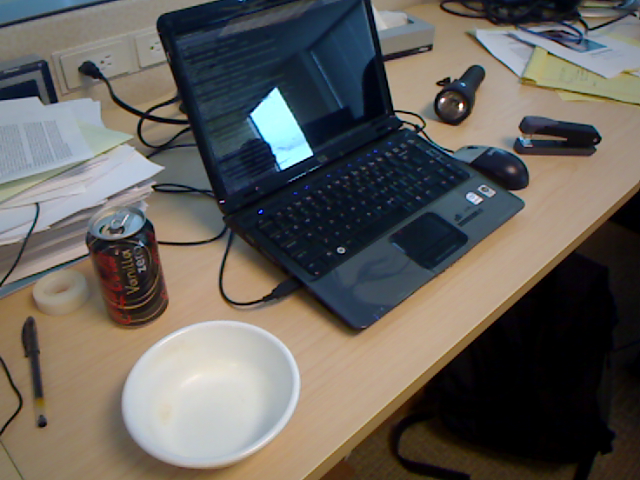
\includegraphics[scale=0.2]{img/escenas/desk_2.png}
        \end{subfigure}

        \begin{subfigure}{0.45\textwidth}
            \centering
            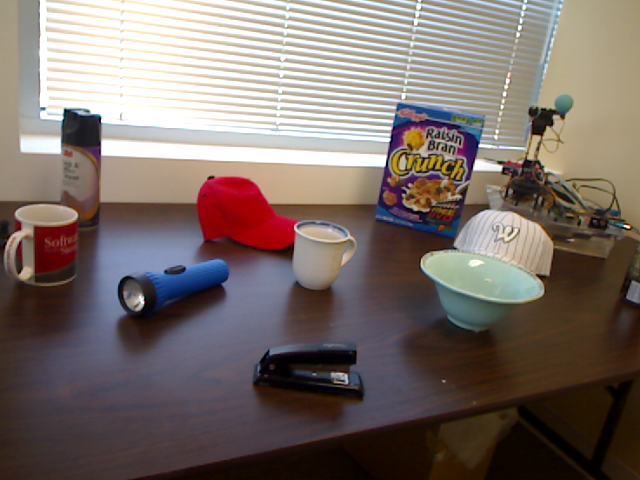
\includegraphics[scale=0.2]{img/escenas/table_1.png}
        \end{subfigure}
        \begin{subfigure}{0.45\textwidth}
            \centering
            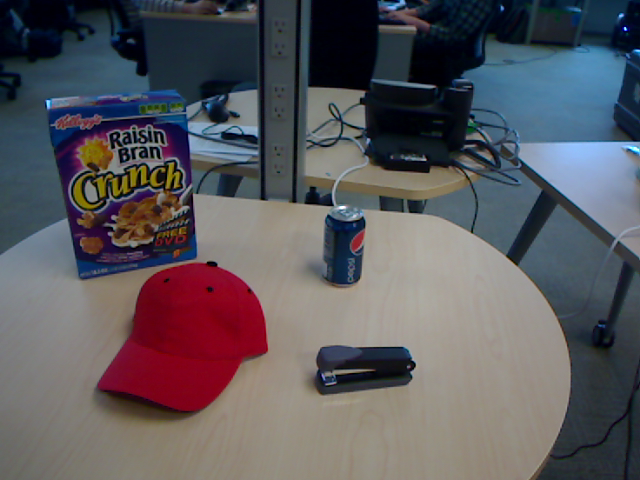
\includegraphics[scale=0.2]{img/escenas/table_small_2.png}
        \end{subfigure}
    \end{figure}
\end{frame}
%--- Next Frame ---%

\subsection{Métricas}
\begin{frame}[t]{Comparación de resultados vs. ground truth}
    \begin{figure}[t]
        \centering
        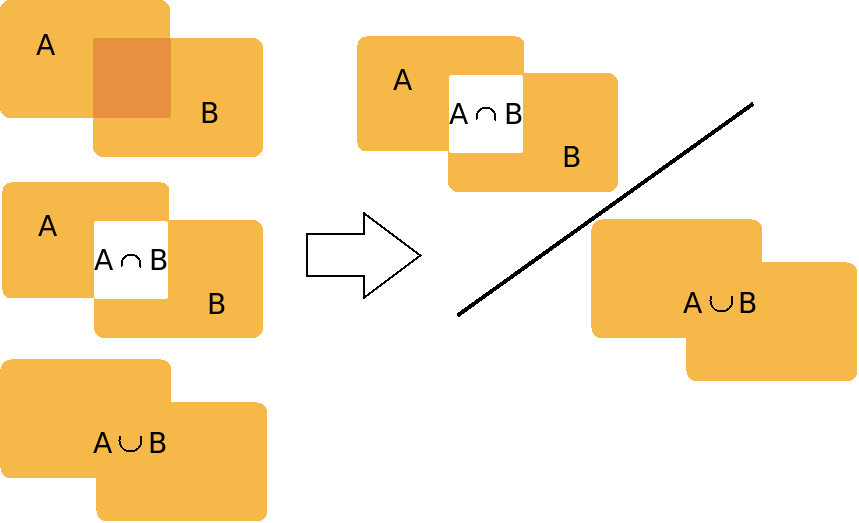
\includegraphics[scale=0.35]{img/pascal/pascal.png}
    \end{figure}
\end{frame}
%--- Next Frame ---%



\subsection{Análisis}
\begin{frame}{Análisis frame por frame para el sistema de profundidad}
    % TODO: poner un gráfico de los de color que se vea bien, junto con el video que salga de ese gráfico y comentar para que sirve analizar el porcentaje de seguimiento, el promedio de solapamiento. Comentar que se usó una detección estática para comparar y analizar solo el comportamiento del seguimiento

    % Cosas para comentar:
    % Este análisis se realizó para los 3 sistemas y para todos los objetos seleccionados.
    % Este gráfico en particular se corresponde con el seguimiento en profundidad de una taza
    % Comentar bien pavo que para los primeros frames hay un solapamiento entre el 50 y 60 %, luego el solapamiento cae a 0. Estos frames en 0 se corresponden con los frames en donde la taza no aparece en la escena. Luego hay una nueva detección y en los frames subsiguientes el solapamiento es aún mejor, llegando a valores entre el 70 y 80 %.
    % De este gráfico surgen varios análisis posibles:
    % 1) Conocer frame a frame la precisión del método de seguimiento
    % 2) Conocer la tasa de seguimiento, es decir, la cantidad de veces que se usa el método de seguimiento
    % 3) Conocer el promedio de solapamiento y tener una idea general de cómo funciona el método (decir como se calcula el promedio de solapamiento)

    Escena $\leftarrow$ Escritorio. Objeto $\leftarrow$ Taza $\dots$ \% de seguimiento: $\sim$ 92
    \vspace*{-15pt}
    \begin{figure}
        \centering
        \includegraphics[scale=0.24]{img/frame_a_frame_depth-taza.png}
    \end{figure}

\end{frame}
%--- Next Frame ---%


\begin{frame}[t]{Comparando seguimientos}
    \small
    % Tablas con el % de seguimiento y solapamiento para RGB, depth y RGB-D
    % Mostrar con colores RGB vs DEPTH. VERDE=GANA, AMARILLO=EMPATA, ROJO=PIERDE
    % Contar que el seguimiento en RGB se ve muy afectado por el fondo y el cambio de colores/luz. La gorra y la caja funcionan bien porque contrastan mucho con el fondo pero el resto de los objetos tienen poca textura y colores cuyo histograma puede confundirse con el del fondo
    % En el caso de profundidad todos funcionan muy parejos salvo la lata y la caja. La lata tiene un modelo muy malo porque refleja la proyeccion infrarroja del sensor y por eso el seguimiento es malo. La caja tiene un buen modelo pero al ser plana no funciona bien.


    % Decir que si no se tiene un método de seguimiento RGB confiable, entonces es preferible utilizar un seguimiento basado únicamente en profundidad

    \begin{columns}
        \begin{column}{4cm}
            \begin{tabular}{|c|c|c|c|}
                \hline    \multirow{6}{*}{\begin{sideways}\parbox{15mm}{RGB}\end{sideways}} & Obj     & \% seg. & \% solap. \\
                \cline{2-4}
                & Taza 1  & \pricomp{red}{47.89}   & \pricomp{red}{34.48}   \\
                \cline{2-4}
                & Gorra   & \pricomp{green}{96.97}   & \pricomp{yellow}{55.68}    \\
                \cline{2-4}
                & Bowl    & \pricomp{red}{6.19}    & \pricomp{red}{12.58}    \\
                \cline{2-4}
                \cline{2-4}
                & Taza 2  & \pricomp{red}{35.9}    & \pricomp{red}{29.54}    \\
                \cline{2-4}
                & Lata    & \pricomp{red}{0}       & \pricomp{red}{0.01}    \\
                \cline{2-4}
                & Caja    & \pricomp{green}{67.62}   & \pricomp{green}{52.11}    \\
                \hline
            \end{tabular}
        \end{column}
        \begin{column}{4cm}
            \begin{tabular}{|c|c|c|c|}
                \hline
                \multirow{6}{*}{\begin{sideways}Profundidad\end{sideways}} & Obj     & \% seg. & \% solap. \\
                \cline{2-4}
                & Taza 1  & \prisegcomp{green}{yellow}{92.16}    & \prisegcomp{green}{yellow}{66.29} \\
                \cline{2-4}
                & Gorra   & \prisegcomp{red}{yellow}{92.67}    & \prisegcomp{yellow}{green}{56.85} \\
                \cline{2-4}
                & Bowl    & \prisegcomp{green}{red}{63.83}    & \prisegcomp{green}{yellow}{40.60} \\
                \cline{2-4}
                \cline{2-4}
                & Taza 2  & \prisegcomp{green}{green}{80.51}   & \prisegcomp{green}{green}{55.79} \\
                \cline{2-4}
                & Lata    & \prisegcomp{green}{red}{10.63}   & \prisegcomp{green}{red}{12.34} \\
                \cline{2-4}
                & Caja    & \prisegcomp{red}{green}{30.62}   & \prisegcomp{red}{green}{44.94} \\
                \hline
            \end{tabular}
        \end{column}
    \end{columns}
    \begin{columns}
        \begin{column}{4cm}
            \begin{tabular}{|c|c|c|c|}
                \hline
                \multirow{6}{*}{\begin{sideways}RGB-D\end{sideways}} & Obj     & \% seg. & \% solap. \\
                \cline{2-4}
                & Taza 1  & \segcomp{yellow}{90.05}   & \segcomp{yellow}{65.07} \\
                \cline{2-4}
                & Gorra   & \segcomp{yellow}{90.82}   & \segcomp{red}{42.83} \\
                \cline{2-4}
                & Bowl    & \segcomp{green}{68.54}   & \segcomp{yellow}{42.88} \\
                \cline{2-4}
                \cline{2-4}
                & Taza 2  & \segcomp{red}{48.33}   & \segcomp{red}{35.98} \\
                \cline{2-4}
                & Lata    & \segcomp{green}{23.67}   & \segcomp{green}{18.81} \\
                \cline{2-4}
                & Caja    & \segcomp{red}{23.29}   & \segcomp{red}{35.03} \\
                \hline
            \end{tabular}
        \end{column}
    \end{columns}
\end{frame}
%--- Next Frame ---%


\begin{frame}[t]{Resultados del sistema RGB-D}
    \small
    $$
    accuracy = \frac{\#TP + \#TN}{\#TP + \#TN + \#FP + \#FN}
    $$
    \normalsize
    \only<1>{
        \begin{table}[h]
        	\centering
            \begin{tabular}{|c|c|c|c|c|c|}
            \hline
            & \multirow{2}{2.4cm}{\% promedio de overlap} & \multirow{2}{2cm}{\% veces ubicado} &\\
        	Objeto & & & Accuracy\\
        	\hline
            Taza    & 50.44      & 76.67     & 83.33 \\
            \hline
            Gorra   & 50.05      & 68.09     & 89.8 \\
            \hline
            Bowl    & 28.18      & 45.67     & 71.4 \\
            \hline
            Taza 2  & 45.54      & 77.78     & 93.07 \\
            \hline
            Lata    & 12.72      & 25.85     & 39.47 \\
            \hline
            Caja    &  6.17      &    10     & 26.92 \\
            \hline
            \end{tabular}
        \end{table}
    }

    \only<2>{
        \begin{table}[h]
        	\centering
            \begin{tabular}{|c|c|c|c|c|c|}
            \hline
            & \multirow{2}{2.4cm}{\% promedio de overlap} & \multirow{2}{2cm}{\% veces ubicado} &\\
        	Objeto & & & Accuracy\\
        	\hline
            Taza    & 50.44      & 76.67     & \cellcolor{green}83.33 \\
            \hline
            Gorra   & 50.05      & 68.09     & \cellcolor{green}89.8 \\
            \hline
            Bowl    & 28.18      & 45.67     & \cellcolor{yellow}71.4 \\
            \hline
            Taza 2  & 45.54      & 77.78     & \cellcolor{green}93.07 \\
            \hline
            Lata    & 12.72      & 25.85     & 39.47 \\
            \hline
            Caja    &  6.17      &    10     & 26.92 \\
            \hline
            \end{tabular}
        \end{table}
    }

    \only<3>{
        \begin{table}[h]
        	\centering
            \begin{tabular}{|c|c|c|c|c|c|}
            \hline
            & \multirow{2}{2.4cm}{\% promedio de overlap} & \multirow{2}{2cm}{\% veces ubicado} &\\
        	Objeto & & & Accuracy\\
        	\hline
            Taza    & \cellcolor{green}50.44      & 76.67     & 83.33 \\
            \hline
            Gorra   & \cellcolor{green}50.05      & 68.09     & 89.8 \\
            \hline
            Bowl    & \cellcolor{red}28.18      & 45.67     & 71.4 \\
            \hline
            Taza 2  & \cellcolor{green}45.54      & 77.78     & 93.07 \\
            \hline
            Lata    & 12.72      & 25.85     & 39.47 \\
            \hline
            Caja    &  6.17      &    10     & 26.92 \\
            \hline
            \end{tabular}
        \end{table}
    }

    \only<4>{
        \begin{table}[h]
        	\centering
            \begin{tabular}{|c|c|c|c|c|c|}
            \hline
            & \multirow{2}{2.4cm}{\% promedio de overlap} & \multirow{2}{2cm}{\% veces ubicado} &\\
        	Objeto & & & Accuracy\\
        	\hline
            Taza    & 50.44      & \cellcolor{yellow}76.67     & 83.33 \\
            \hline
            Gorra   & 50.05      & \cellcolor{yellow}68.09     & 89.8 \\
            \hline
            Bowl    & 28.18      & \cellcolor{red}45.67     & 71.4 \\
            \hline
            Taza 2  & 45.54      & \cellcolor{yellow}77.78     & 93.07 \\
            \hline
            Lata    & 12.72      & 25.85     & 39.47 \\
            \hline
            Caja    &  6.17      &    10     & 26.92 \\
            \hline
            \end{tabular}
        \end{table}
    }

\end{frame}
%--- Next Frame ---%






%%%%%%%%%%%%%%%%%%%%%%%%%%
%%%%%%%%%%%%%%%%%%%%%%%%%%
\section{Conclusiones y trabajo a futuro}
\begin{frame}{Conclusiones y trabajo a futuro}
    \begin{itemize}
        \item Buena tasa de seguimiento con un modelo sencillo
        \item Seguimiento en profundidad robusto y con bajas tasas de falsos positivos
        \item Muy importante tener un método de detección robusto y preciso
        \item El método podría funcionar en escenas en donde tanto los objetos como la cámara se mueven
        \item Implementar un algoritmo robusto frente a oclusiones (ej: usar filtro de Kalman)
    \end{itemize}
\end{frame}
%--- Next Frame ---%

\begin{frame}[t]{¿Preguntas?}
    \begin{figure}
        \centering
        \includegraphics[scale=0.5]{img/preguntas.jpg}
    \end{figure}
\end{frame}
%--- Next Frame ---%


\begin{frame}[t]{¡Muchas gracias a todos!}
    \vspace{-20pt}
    \begin{figure}
        \centering
        \hspace*{-18pt}\includegraphics[scale=0.2]{img/gracias.jpg}
    \end{figure}
\end{frame}
%--- Next Frame ---%


\end{document}


% TODO: Preguntar a Pachi si está bien esto: la detección/seguimiento en RGB no es facilmente utilizable para detectar objetos de una misma clase (no distinguir instancias sino clase de objetos) ya que en general dos objetos de la misma categoría pueden no compartir los mismos colores y esa información que pueden no compartir es justamente de la que se valen los metodos RGB para detectar/seguir un objeto. En template matching si se quieren detectar categorías se debería proveer al método de templates de todas las instancias que se pueden llegar a encontrar.
% En profundidad en cambio, como en general los objetos de la misma categoría comparten forma, se puede llegar a detectar un objeto dentro de una categoría para el cual no se haya entrenado el método de detección/seguimiento.
